\documentclass[aspectratio=169,kulak,t,handout]{kulakbeamer} % handout

\usepackage{pgfplotstable}
\usepackage{tikz}
\usetikzlibrary{positioning}
\usepackage{hyperref}
\usepackage[dutch]{babel}
\usepackage[T1]{fontenc}
\usefonttheme[onlymath]{serif}

\title[Groep 1 - Safety First]{Miniatuurrobotwagen in een Smart City}
\subtitle{Probleemoplossen en ontwerpen, deel 2}
\author{Camille Louagie, Emiel Vanspranghels, Otto Meerschman, Ruben Leenknecht, Staf Rys}
 
\institute[Kulak]{KU Leuven Kulak}
\date{Academiejaar 2020 -- 2021}

\AtBeginSection[]{\only<beamer>{\addtocounter{framenumber}{-1}
		\begin{outlineframe}\frametitle{Overzicht}
			\tableofcontents[currentsection,hideallsubsections]
	\end{outlineframe}}}

\linespread{1.2}
\setbeamertemplate{frametitle}
{
	\vspace{18pt}
	{\large\textbf{\insertframetitle}} 
}
\begin{document}

\begin{titleframe}
\titlepage
\end{titleframe}


\section*{Probleemstelling en oplossing}

\begin{frame}
	\frametitle{\Large Verdere verstedelijking creëert mobiliteitsproblemen.}


	\begin{figure}
		\centering
		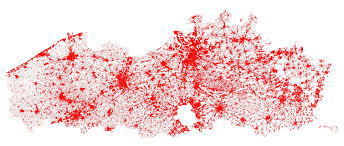
\includegraphics[width=.6\textwidth]{ruimtelijkestaat}
		%rood= ruimtebeslag > drempelwaarde
		
		\label{fig:ruimtelijkestaat}
	\end{figure}
	\begin{itemize}
	\item  De files stijgen gemiddeld met gemiddeld 2\% per jaar (voor Corona)
	\item  Steden (0.5\% van de aardoppervlakte) consumeren 75\% van de natuurlijke middelen
\end{itemize}

\end{frame}

\begin{frame}
	\frametitle{{\Large Slimme steden als oplossing voor het mobiliteitsprobleem}}
	
\begin{block}{Definitie}
	
	Een stad die technologische innovatie gebruikt om de stedelijke werking efficiënt te laten verlopen
	
\end{block}	
	\begin{itemize}
		\large\item  Heeft als doel het verbeteren van interacties
		\begin{itemize}
			\normalsize\item Door op te wegen tegen fysieke beperkingen
			\item Door de levenskwaliteit te verhogen
		\end{itemize}
		\item  (Openbare) diensten vereenvoudigen
	\end{itemize}
\end{frame}



\begin{frame}{{\Large Wegen de voordelen van zelfrijdende auto's op tegen de nadelen?}}
	\begin{columns}
	\column{0.5\textwidth}\centering
	{\bf{Voordelen}}\\[.2cm]

		\begin{itemize}
			\large\item Minder ongevallen
			\begin{itemize}
				\normalsize\item Auto's kennen de nabije buren
				\item Dynamische snelheidsaanpassing
			\end{itemize}
			\item Respect voor de verkeersregels
			\item Tijd van de bestuurder word vrijgemaakt
			
		\end{itemize}
	\column{0.5\textwidth}\centering
	{\bf{Nadelen}}\\[.2cm]

			\begin{itemize}
			\large\item Kwetsbaar voor hackers
			\item Daling overheidsinkomsten
			\item Stijging werkeloosheid
			\item Juridische conflicten door aansprakelijkheid bij ongevallen
			\end{itemize}
	
	\end{columns}
\end{frame}

\begin{outlineframe}[Overzicht]
	\tableofcontents
\end{outlineframe}


\section{Ontwerpspecificaties}

\begin{frame}{\Large Negen kruispunten vormen een modelstad.}
	
	\begin{tikzpicture}
		\node [anchor=west] (Volglijn met stopstreep) at (-2,0.8) {\Large Volglijn met stopstreep};
		\node [anchor=west] (verkeerslicht) at (-2,2.5) {\Large Verkeerslicht};
		\tikzstyle{every node}=[fill=red!20,rounded corners]
		\node [anchor=west] (Weg) at (11.25,3.2) {\large 250 mm};
		\begin{scope}[xshift=1.5cm]
			\tikzstyle{every node}=[fill=red!20,rounded corners]
			\node[anchor=south west,inner sep=0] (image) at (2,0) {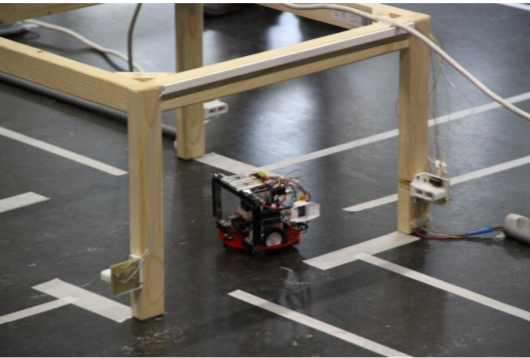
\includegraphics[width=0.5\textwidth]{modelstad}};
			\node [anchor=west] (Afstand) at (8.75,1.8) {\large 75 mm};
			\begin{scope}[x={(image.south east)},y={(image.north west)}]
				%\draw[cyan,ultra thick,rounded corners] (0.4,0.55) rectangle (0.2,0.3);
				\draw [-stealth, line width=3pt, cyan] (Volglijn met stopstreep) -- ++(0.43,0.0);
				%\draw[cyan,ultra thick,rounded corners] (0.4,0.55) rectangle (0.2,0.3);
				\draw [-stealth, line width=3pt, cyan] (verkeerslicht) -- ++(1.05,0.0);
			\end{scope}
				\draw[thick,red,->,line width=0.5mm] (8.5,1.65) -- (8.5,2.5);
				\draw[thick,red,->,line width=0.5mm] (8.5,2.5) -- (8.5,1.65);
				\draw[thick,red,->,line width=0.5mm] (9.5,2.2) -- (9.5,3.65);
				\draw[thick,red,->,line width=0.5mm] (9.5,3.65) -- (9.5,2.2);
		\end{scope}
	\end{tikzpicture}
\end{frame}






\section{Ontwerp}

\begin{frame}{\Large Sensoren laten ons toe om informatie van de wereld in te lezen.}
\noindent
\begin{tikzpicture}
	\node [anchor=west] (Lijnsensor) at (-2,1) {\Large Lijnsensor};
	\node [anchor=west] (Kleurensensor) at (-2,5.5) {\Large Kleurensensor};
	\node [anchor=west] (Afstandssensor) at (-2,2.25) {\Large Afstandssensor};
	\begin{scope}[xshift=1.5cm]
		\node[anchor=south west,inner sep=0] (image) at (0,0) {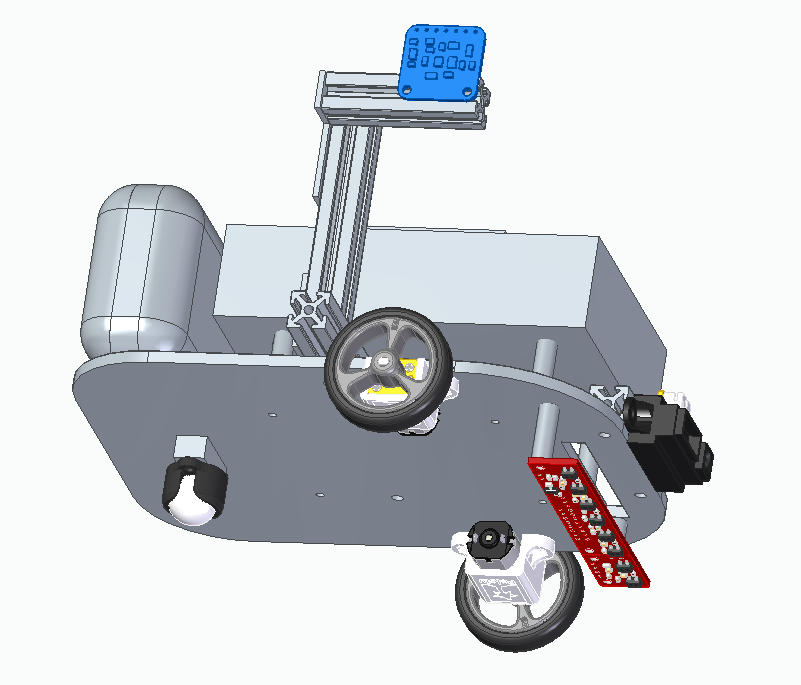
\includegraphics[width=0.5\textwidth]{OAZ}};
		\begin{scope}[x={(image.south east)},y={(image.north west)}]
			%\draw[cyan,ultra thick,rounded corners] (0.4,0.55) rectangle (0.2,0.3);
			\draw [-stealth, line width=3pt, cyan] (Lijnsensor) -- ++(1.06,0.0);
			%\draw[cyan,ultra thick,rounded corners] (0.4,0.55) rectangle (0.2,0.3);
			\draw [-stealth, line width=3pt, cyan] (Kleurensensor) -- ++(0.77,0.0);
			\draw [-stealth, line width=3pt, cyan] (Afstandssensor) -- ++(1.05,0.0);
		\end{scope}
	\end{scope}
\end{tikzpicture}
\end{frame}


\begin{frame}{\Large De microcontroller gebruikt de ingelezen data om gepast te reageren.}
\noindent
\begin{tikzpicture}
	\node [anchor=west] (Microcontroller) at (-1,3) {\Large Microcontroller};
	\node [anchor=west] (Batterij) at (-1,5) {\Large Batterij};
	\begin{scope}[xshift=1.5cm]
		\node[anchor=south west,inner sep=0] (image) at (1,0) {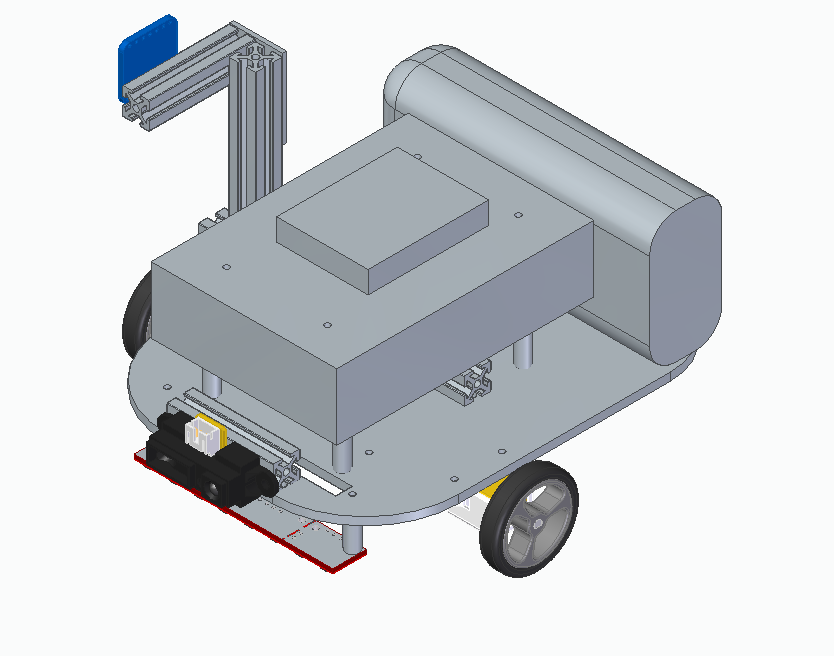
\includegraphics[width=0.55\textwidth]{6.PNG}};
		\begin{scope}[x={(image.south east)},y={(image.north west)}]
			%\draw[cyan,ultra thick,rounded corners] (0.4,0.55) rectangle (0.2,0.3);
			\draw [-stealth, line width=3pt, cyan] (Microcontroller) -- ++(0.5,0.0);
			%\draw[cyan,ultra thick,rounded corners] (0.4,0.55) rectangle (0.2,0.3);
			\draw [-stealth, line width=3pt, cyan] (Batterij) -- ++(0.85,0.0);
		\end{scope}
	\end{scope}
\end{tikzpicture}	
\end{frame}

\begin{frame}{\Large De sensoren en processoren worden geplaatst op een zelf-ontworpen chassis.}
	\noindent
	\begin{tikzpicture}
		\node [anchor=west] (Wiel) at (-1,3.5) {\Large Wiel};
		\node [anchor=west] (Chassis) at (-1,2.5) {\Large Chassis};
		\node [anchor=west] (Kogelrol) at (-1,1) {\Large Kogelrol};
		\begin{scope}[xshift=1.5cm]
			\node[anchor=south west,inner sep=0] (image) at (1,0) {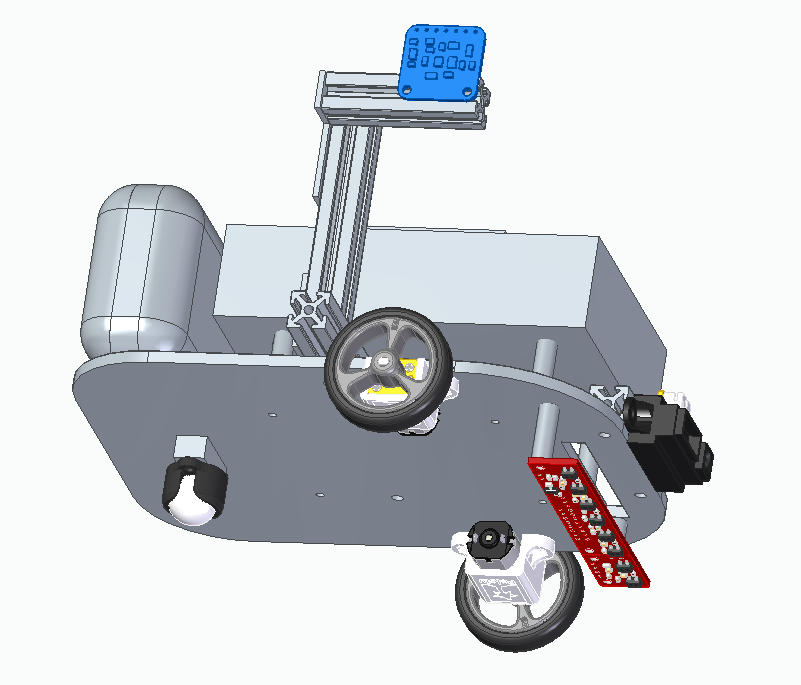
\includegraphics[width=0.50\textwidth]{OAZ}};
			\begin{scope}[x={(image.south east)},y={(image.north west)}]
				%\draw[cyan,ultra thick,rounded corners] (0.4,0.55) rectangle (0.2,0.3);
				\draw [-stealth, line width=3pt, cyan] (Wiel) -- ++(0.73,-0.1);
				%\draw[cyan,ultra thick,rounded corners] (0.4,0.55) rectangle (0.2,0.3);
				\draw [-stealth, line width=3pt, cyan] (Chassis) -- ++(0.45,0.0);
				\draw [-stealth, line width=3pt, cyan] (Kogelrol) -- ++(0.47,0.1);
			\end{scope}
		\end{scope}
	\end{tikzpicture}	
\end{frame}


\begin{frame}{\Large Verschillende keuzes werden gemaakt bij het ontwerpen van het chassis.}
	
	\begin{tikzpicture}
	
		\tikzstyle{every node}=[fill=red!20,rounded corners]
		\begin{scope}[xshift=1.5cm]
			\tikzstyle{every node}=[fill=red!20,rounded corners]
			\node[anchor=south west,inner sep=0] (image) at (6,0) {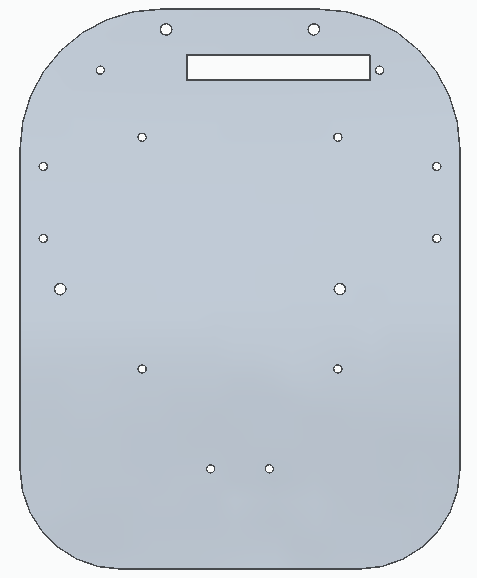
\includegraphics[width=0.3\textwidth]{chascad}};
			\node [anchor=west] (breedte) at (7.3,0.3) {\large 110 mm};
			\node [anchor=west] (lengte) at (6.2,2.5) {\large 140 mm};
			\draw[thick,red,->,line width=0.5mm] (6.0,0) -- (6.0,5.1);
			\draw[thick,red,->,line width=0.5mm] (6.0,5.1) -- (6.0,0);
			\draw[thick,red,->,line width=0.5mm] (10.2,-0.2) -- (6.3,-0.2);
			\draw[thick,red,->,line width=0.5mm] (6.3,-0.2) -- (10.2,-0.2);
			\begin{scope}[x={(image.south east)},y={(image.north west)}]
				%\draw[cyan,ultra thick,rounded corners] (0.4,0.55) rectangle (0.2,0.3);
				%\draw [-stealth, line width=3pt, cyan] (Volglijn met stopstreep) -- ++(0.43,0.0);
				%\draw[cyan,ultra thick,rounded corners] (0.4,0.55) rectangle (0.2,0.3);
				%\draw [-stealth, line width=3pt, cyan] (verkeerslicht) -- ++(1.05,0.0);
			\end{scope}

		\end{scope}
		\begin{scope}[xshift=1.5cm]
			\tikzstyle{every node}=[fill=red!20,rounded corners]
			\node[anchor=south west,inner sep=0] (image) at (15,0) {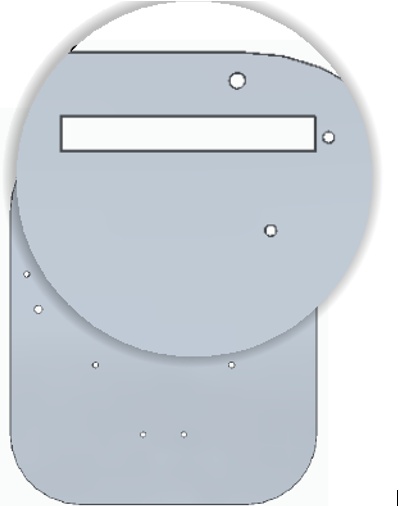
\includegraphics[width=0.3\textwidth]{zoom}};
			\node [anchor=west] (breedte) at (13.3,3.9) {\large 6.5 mm};
			\node [anchor=west] (lengte) at (16.2,3.1) {\large 45.8 mm};
			\draw[thick,red,->,line width=0.5mm] (15.5,3.9) -- (15.5,4.3);
			\draw[thick,red,->,line width=0.5mm] (15.5,4.3) -- (15.5,3.9);
			\draw[thick,red,->,line width=0.5mm] (15.7,3.6) -- (18.5,3.6);
			\draw[thick,red,->,line width=0.5mm] (18.5,3.6) -- (15.7,3.6);
			\begin{scope}[x={(image.south east)},y={(image.north west)}]
			%\draw[cyan,ultra thick,rounded corners] (0.4,0.55) rectangle (0.2,0.3);
			%\draw [-stealth, line width=3pt, cyan] (Volglijn met stopstreep) -- ++(0.43,0.0);
			%\draw[cyan,ultra thick,rounded corners] (0.4,0.55) rectangle (0.2,0.3);
			%\draw [-stealth, line width=3pt, cyan] (verkeerslicht) -- ++(1.05,0.0);
			\end{scope}
		
		\end{scope}
\end{tikzpicture}

\end{frame}



\section{Evaluatie}

\begin{frame}{\Large Besluit}
\begin{itemize}
	\large \item Zelfrijdend wagentje: Legt zo goed als probleemloos een parcours af
	\item Toont mogelijkheden op grote schaal
	\item Budgetoverschot: Veiling anders aanpakken of meer 3D-printen
	
\end{itemize}	
	
\end{frame}

\begin{frame}{\Large De demo}
\begin{columns}
	\column{0.4\textwidth}\centering
	
		\begin{figure}
			\centering
			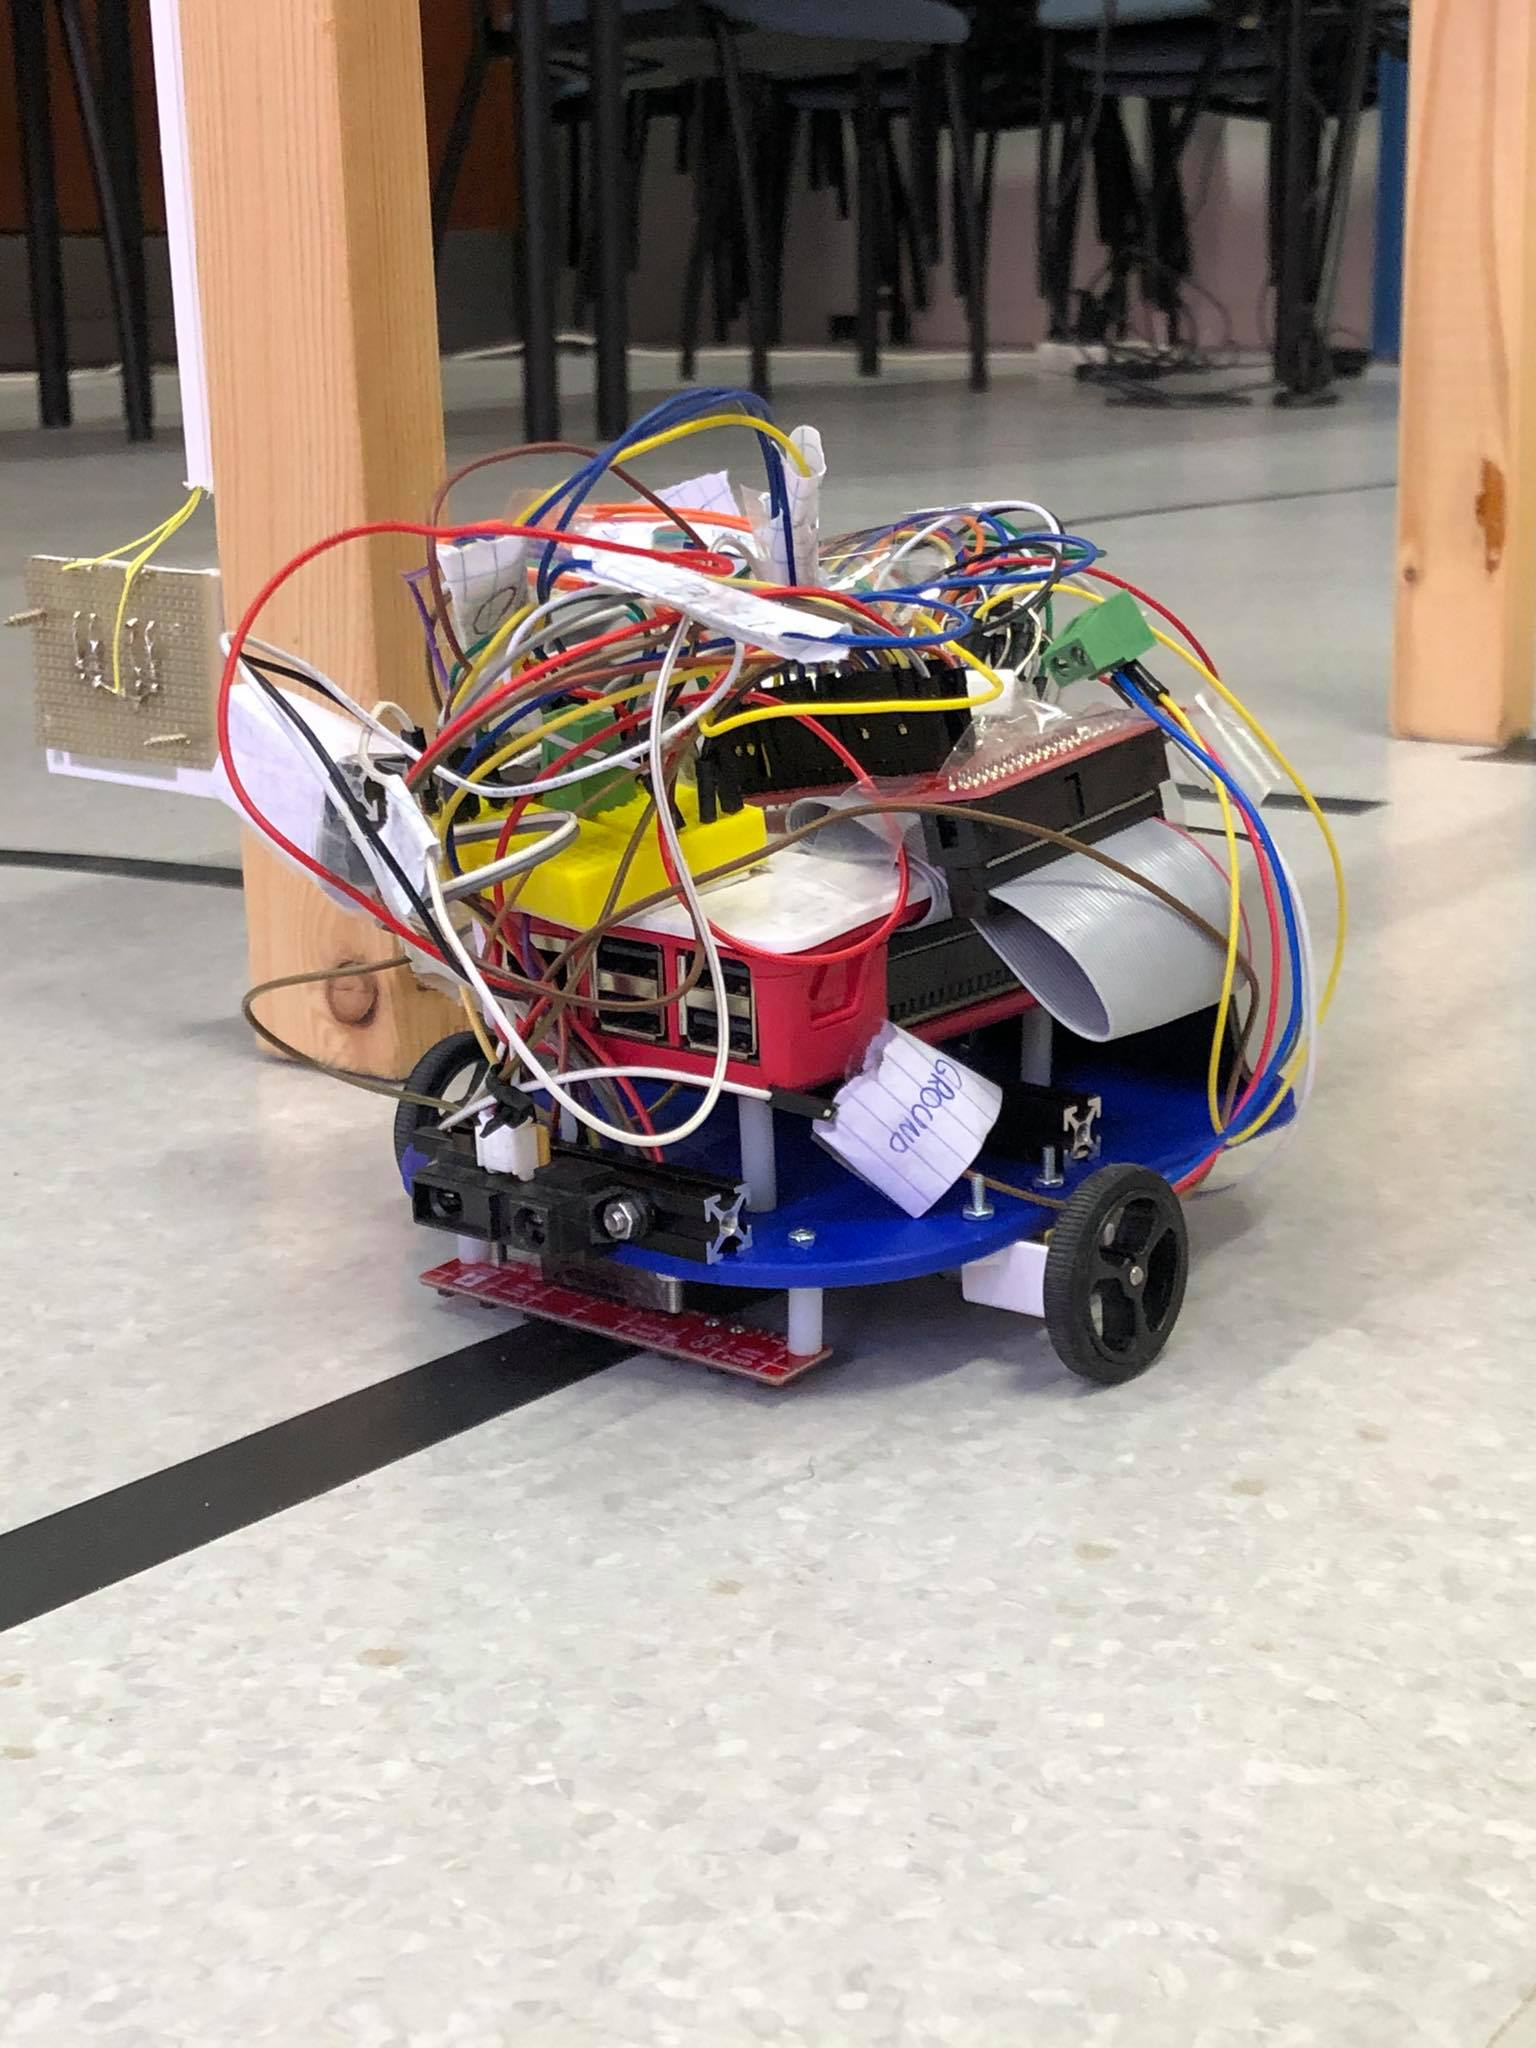
\includegraphics[width=.5\textwidth]{demo}
			%rood= ruimtebeslag > drempelwaarde
			
			\label{fig:Demo}
		\end{figure}
	\column{0.6\textwidth}\centering
	{\bf{Conclusies getrokken na de demo}}\\[.2cm]
	
	\begin{itemize}
		\large\item Er is een grotere minimumafstand bij de afstandssensor nodig.
		\item Iets 3D-printen voor rond de kleurensensor in plaats van papier
		\item Het kabelmanagement verfijnen
	\end{itemize}
	
\end{columns}

	
\end{frame}

\begin{frame}{\Large De financiële situatie}

\begin{centering}
	\begin{tikzpicture}
		
		
		
		\pgfplotstableread[row sep=\\]{ % Read the data into a table macro
			Label                                      First   \\
			{Motor} 									  640	\\
			{Sensoren} 									 460	\\
			{Makerbeams}  								 115	\\
			{Chassis} 									120		\\
			{Microcontroller}							 240	\\
			{Powerbank}									 180	\\
			%{Wireframes}                                 0     \\
		}\datatable
		
		\begin{axis}[
			xbar stacked,   % Stacked horizontal bars
			xmin=0,  xmax=700,       % Start x axis at 0
			%title={\large \textbf {Gantt Chart }},
			height=7cm, width=8cm,
			bar width=0.7cm,
			axis x line*=bottom,
			axis y line*=left,
			y axis line style={opacity=1},
			enlarge y limits=true,
			xmajorgrids={true},
			grid style={
				solid,
				ultra thin,
				gray
			},
			tick style={tickwidth=0cm,major tick length=0cm},
			xlabel={\textbf{Kredietpunten}},
			xtick ={100,200,300,400,500,600},
			%xminorgrids={true},
			%grid style={
			%dashed,
			%   ultra thin,
			%   gray
			%   },
			%minor xtick ={1,3,5,7,9,11,13,15},
			%grid =both,
			yticklabel style={font=\small\bfseries},
			ytick=data,     % Use as many tick labels as y coordinates
			yticklabels from table={\datatable}{Label}  % Get the labels from the Label column of the \datatable
			]
			\addplot [draw=none,fill=blue] table [x=First, y expr=\coordindex] {\datatable};    % Plot the "First" column against the data index
			\addplot [draw=none,fill=red]table [x=Second, y expr=\coordindex] {\datatable};
			
			
		\end{axis}
		
		
	\end{tikzpicture}
	
\end{centering}
	
\end{frame}

	
\section*{Referenties}

\begin{frame}[allowframebreaks]
	\frametitle{\Large Referenties}
	\nocite{*}
	\bibliographystyle{amsalpha}
	\bibliography{bibliografietv.bib}
\end{frame}


\begin{frame}
	\begin{table}
		\centering
		
		\begin{tabular}{|l|r|r|r|}\hline
			\textbf{Motor}&	\textbf{toeren/min} &	\textbf{km/h}	\\\hline
			100:1 HP&	310&	0.78\\\hline
			100:1&	130&	1.87 	\\\hline
			50:1 HP&	590&	2.71 \\\hline
			30:1&	1000&	3.56	\\\hline
			30:1 HP&	450&	6.03 	\\\hline
		\end{tabular}
		\caption{Berekening snelheid voor elke motor voor wielen met diameter 32 mm}\label{MotorenTab}
		
	\end{table}
\end{frame}

\begin{frame}
	\begin{tikzpicture}
	
	\tikzstyle{every node}=[fill=red!20,rounded corners]
	\begin{scope}[xshift=1.5cm]
		\tikzstyle{every node}=[fill=red!20,rounded corners]
		\node[anchor=south west,inner sep=0] (image) at (4,0) {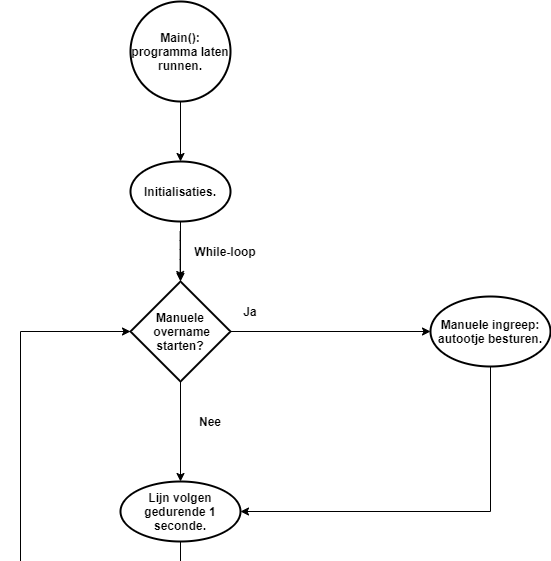
\includegraphics[width=0.5\textwidth]{bovenste}};

		\begin{scope}[x={(image.south east)},y={(image.north west)}]
			%\draw[cyan,ultra thick,rounded corners] (0.4,0.55) rectangle (0.2,0.3);
			%\draw [-stealth, line width=3pt, cyan] (Volglijn met stopstreep) -- ++(0.43,0.0);
			%\draw[cyan,ultra thick,rounded corners] (0.4,0.55) rectangle (0.2,0.3);
			%\draw [-stealth, line width=3pt, cyan] (verkeerslicht) -- ++(1.05,0.0);
		\end{scope}
		
	\end{scope}
	\begin{scope}[xshift=1.5cm]
		\tikzstyle{every node}=[fill=red!20,rounded corners]
		\node[anchor=south west,inner sep=0] (image) at (12,0) {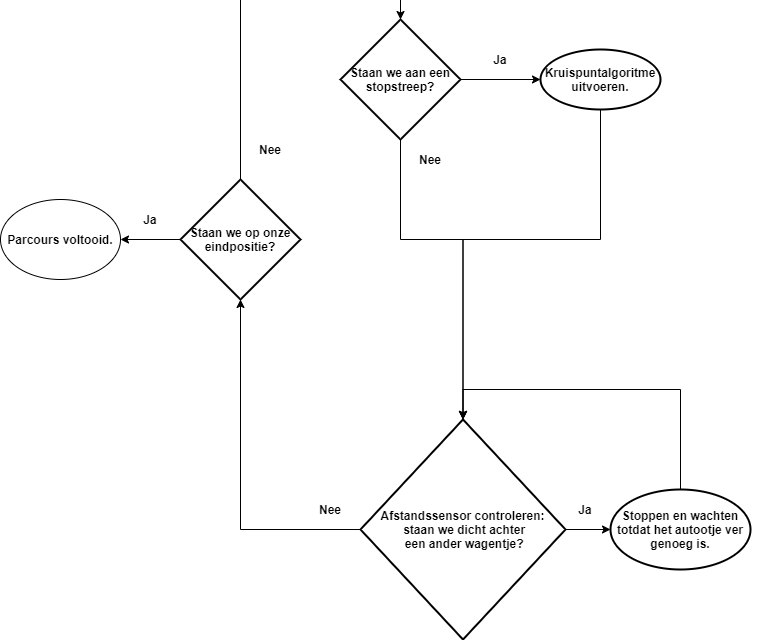
\includegraphics[width=0.5\textwidth]{onderste}};
		\begin{scope}[x={(image.south east)},y={(image.north west)}]
			%\draw[cyan,ultra thick,rounded corners] (0.4,0.55) rectangle (0.2,0.3);
			%\draw [-stealth, line width=3pt, cyan] (Volglijn met stopstreep) -- ++(0.43,0.0);
			%\draw[cyan,ultra thick,rounded corners] (0.4,0.55) rectangle (0.2,0.3);
			%\draw [-stealth, line width=3pt, cyan] (verkeerslicht) -- ++(1.05,0.0);
		\end{scope}
		
	\end{scope}
\end{tikzpicture}
		
\end{frame}


\end{document}